\chapter{Background and Related Work}
\label{chap:background}
Einführung in das kapitel \cite{NOT FINAL}
 \section{Robot-in-the-Loop-Testing}
\label{sec:RitL}
The validation and verification of modern Robotic and Autonomous Systems (RAS) is a significant challenge due to their complexity \cite{AMV23}. This is because they integrate software, mechanical, and electrical engineering all at once \cite{AMV23}. A central problem is ensuring that the software and hardware work together seamlessly, especially when testing both simultaneously \cite{AMV23}. The X-in-the-Loop (XitL) simulation paradigm addresses this challenge \cite{Brayanov2019}. It offers a way to combine the flexibility of software simulation with the realism of physical experiments \cite{Brayanov2019}.

A foundational XitL method is Hardware-in-the-Loop (HIL) simulation, which is a technique for testing mechatronic systems \cite{Mihalic2022, Brayanov2019}. The main principle of HIL is creating a closed loop between the real hardware that is being tested and a simulation that represents the rest of the system or its operational environment \cite{Mihalic2022}. This setup effectively tricks the hardware into behaving as if it were operating in a real system, which allows for testing across a wide range of virtual scenarios \cite{Brayanov2019}. The main reason for using HIL is to shorten development cycles and prevent costly or dangerous failures by making exhaustive testing possible before the system is actually completely implemented \cite{Mihalic2022}.This is why HIL is essential in industries like automotive, aerospace, and robotics, where real-world testing can be too expensive, dangerous, or even impossible \cite{Brayanov2019}.

Robot-in-the-Loop (RitL) \cite{Mihalic2022} simulation extends the Hardware-in-the-Loop (HIL) concept. Instead of just a component, the hardware under test is a complete robotic system, such as an uncrewed vehicle \cite{Mihalic2022}. RitL replaces components of an pure simulated setup with the actual robot, increasing the realism of testing \cite{Hu05}. \cite{NOT FINAL}As illustrated in Figure \ref{fig:ritl_concept}\cite{NOT FINAL}, a typical RitL configuration has the robot's real actuators operating in the physical world, while while its sensors interact with a simulated environment instead \cite{Hu05, Mihalic2022}. This creates a hybrid setup where, for example, the robot might use virtual sensors to see objects in the simulation but use its real motors to move physically \cite{Hu05}. To keep the physical and virtual worlds synchronized, the real robot often has a virtual counterpart in the simulation which state is updated as the physical robot acts and moves \cite{Hu05}.

\begin{figure}[h]
\centering
% \includegraphics[width=0.8\textwidth]{path/to/ritl_concept_diagram.png}
\caption{\cite{NOT FINAL}The real robot's actions affect its virtual counterpart, and the virtual environment provides sensor data back to the real robot.\cite{NOT FINAL}}
\label{fig:ritl_concept}
\end{figure}

The main benefit of RitL is that it uses the dynamics of actual hardware for repeatable testing of high-level software, such as navigation algorithms \cite{Mihalic2022}. This method avoids the expense, complexity, and risk of full physical testbeds while being a secure and useful substitute \cite{Mihalic2022}. RitL becomes therefore an tool for safely evaluating system performance in the lab \cite{Hu05, Mihalic2022}. This is especially important when working on projects that are hard to replicate, such as large-scale robot swarms or Mars rover missions, or when safety is at risk \cite{Hu05, Mihalic2022}.

The RitL paradigm has been widely applied to validate complex autonomous systems, particularly in the automotive field using Vehicle-in-the-Loop (VitL) testing. For example, the Dynamic Vehicle-in-the-Loop (DynViL) architecture integrates a real test vehicle with the high-fidelity CARLA simulator, which operates on the Unreal Engine \cite{DSR22}. As shown in Figure \ref{fig:vitl_setup}, this approach allows a vehicle on an empty track to be stimulated by sensor data from a virtual world \cite{DSR22}. This lets automated driving functions to be safely and reliably tested in situations that would be hazardous to physically replicate \cite{DSR22}. CARLA and the Unreal Engine are also used in a similar Vehicle-in-Virtual-Environment (VVE) method which establishes a closed loop in which the motion of the real vehicle is tracked and reflected in the virtual world, making it possible its control systems to respond to simulated events \cite{Cao2023}.

\begin{figure}[h]
\centering
\includegraphics[width=0.9\textwidth]{images/vehicle_in_the_loop_dsr+22.jpg}
\caption{An example of a Vehicle-in-the-Loop (VitL) setup. A real car on a test track connected to a high-fidelity simulator like CARLA that generates virtual traffic and sensor data. \cite{DSR22}}
\label{fig:vitl_setup}
\end{figure}

These examples show a trend towards using game engine based simulators to evaluate autonomous vehicles. This method falls somewhere between physical testing, where safety and consistency can be problematic, and pure software simulation, which frequently lacks vehicle dynamics fidelity \cite{Cao2023}. Some systems even stimulate the vehicle’s actual sensors. For instance, the Radar Target Simulator (RTS) can feed artificial radar echoes from a virtual scene to the vehicle's actual radar sensor \cite{Diewald2021}. This allows for end-to-end validation of the entire perception and control pipeline \cite{Diewald2021}.

The X-in-the-Loop approach is found in many different areas, not just a single field. In marine robotics, a VIL framework was developed to test the long term autonomy of a robot swarm. In this system, an Autonomous Surface Vehicle (ASV) interacts with multiple simulated underwater sensor nodes to test cooperative behaviors without the logistical cost of deploying a full swarm \cite{Babic2020}. In the aerospace domain, the RFlySim platform uses an FPGA-based HIL system to create a high fidelity simulation for testing UAV autopilot systems in a lab, which reduces the need for expensive and risky outdoor flights \cite{Dai2021}.

These approaches continue to move toward deeper integration. This includes the introduction of Scenario-in-the-Loop (SciL) frameworks that aim to completely blur the lines between real and virtual testing \cite{Szalay2021}. These systems rely on creating detailed digital twins of the entire test environment and combining real and virtual components to run complex, mixed reality test scenarios \cite{Szalay2021}.

\section{Digital Twins}
\label{sec:DT}
The Digital Twin (DT) is an important concept in many current X-in-the-Loop frameworks. The DT serves as the virtual counterpart to a physical system, acting as a virtual copy that allows real-time monitoring and simulation \cite{AA23}. The idea is to create a digital information model of a physical system that stays linked to it for the duration of its lifecycle \cite{Grieves2017}.

This concept was initially known as the Information Mirroring Model and consists of three core elements: the physical product, its corresponding virtual model, and the data connection that connects them \cite{Grieves2017, AA23}. A diagram of this structure is shown in Figure \ref{fig:dt_concept}. The virtual model is more than a basic geometric shape, it is often a detailed simulation that can model mechanical, electrical, and software properties of a system \cite{Leng2021}. Information moves in both directions, so sensor data can flow from the real world to update the virtual model \cite{Grieves2017, Leng2021}. In turn, the virtual model can also send commands back to control or optimize the physical system \cite{Grieves2017, Leng2021}. This continuous, bidirectional data exchange characterizes a Digital Twin \cite{AA23}.

\begin{figure}[h]
\centering
\includegraphics[width=0.8\textwidth]{images/info_mirror_model_Grieves15.png}
\caption{The foundational concept of a Digital Twin, illustrating the three core components: the physical entity, the virtual model, and the bi-directional data connection that links them \cite{Grieves2017, Leng2021}. \cite{Grieves15}}
\label{fig:dt_concept}
\end{figure}

Digital Twins in robotics are frequently created using simulation software and the middleware that connects the virtual simulation to the actual hardware is often the Robot Operating System (ROS) \cite{MFG22}. Stączek et al. used the Gazebo simulator with ROS to create a DT of a factory floor, which they used to test and optimize the navigation algorithms of a mobile robot in narrow corridors \cite{Staczek2021}.  To validate a deep learning-based harvesting robot, R. Singh et al. adopted a similar strategy and created a DT of a greenhouse in Gazebo \cite{Singh2024a}. Other simulators like CoppeliaSim and Webots are also common. Magrin et al. used CoppeliaSim and ROS to create a DT as a learning tool for mobile robot design \cite{Magrin2021}, while Marques et al. used Webots for an Automated Guided Vehicle (AGV), synchronizing it via an OPC-UA server \cite{Marques2024}. These examples show a common approach of using traditional simulators to simulate robot kinematics and sensor feedback for closed-loop testing.

More recently, game engines have become a popular choice for creating Digital Twins, as they offer more realistic graphics and physics. Unity \cite{Uni23}, for instance, is used developers to build virtual environments that are highly realistic. \cite{NOT FINAL}This can be seen in Figure \ref{fig:dt_environments}\cite{NOT FINAL}. Pérez et al. used Unity to develop a DT of a multi-robot cell with a Virtual Reality (VR) interface for virtual commissioning and operator training \cite{Perez2020}.

\begin{figure}[h]
\centering
% \includegraphics[width=0.9\textwidth]{path/to/dt_environments_comparison.png}
\caption{\cite{NOT FINAL}A comparison of robotic Digital Twin environments, showing a view from a traditional simulator (left) versus a high-fidelity visualization from a modern game engine like Unity (right).\cite{NOT FINAL}}
\label{fig:dt_environments}
\end{figure}

Another important consideration are the technical capabilities these engines. Yang et al. \cite{Yang2020} simulated the physics of a UAV using Unity and its built-in NVIDIA PhysX engine. They also demonstrated the creation of virtual sensors, such as a LiDAR, directly within the game engine using its raycasting API \cite{Yang2020}. Research has also been done on the performance and reliability of these game engine-based frameworks. Kwon et al. developed a safety-critical DT in Unity and ROS 2, reaching a data-transmission latency of 13 ms for predicting collisions \cite{Kwon2025}. Similarly, M. Singh et al. created a DT using ROS and Unityand and conducted performance validation with a communication latency of 77.67 ms and a positional accuracy of 99.99\% \cite{Singh2024b}.

\section{Mixed Reality}
\label{sec:MR}
Beyond the testing paradigm and the digital twin, the way a user interacts with the system is another part of a modern robotics framework. Virtual, Augmented, and Mixed Reality (VAM) have become promising technologies for improving the information exchange between humans and robots \cite{Walker2023}. In robotics, Augmented Reality (AR) is an especially useful tool for enhancing Human-Robot Interaction (HRI) by integrating 3D virtual objects into a real-world environment in real-time \cite{MV20}.

The relationship between these technologies is formally described by the foundational Reality-Virtuality (RV) Continuum concept, first introduced by Milgram and Kishino \cite{MK94}. As illustrated in Figure \ref{fig:rv_continuum}, this continuum is a scale that is anchored by a purely real environment at one end and a completely virtual one at the other \cite{MK94, Skarbez2021, MV20}.

\begin{figure}[h]
\centering
\includegraphics[width=0.9\textwidth]{images/reality_virtuality_continuum_wpc+23.png}
\caption{The Reality-Virtuality Continuum, illustrating the spectrum from a real environment to a completely virtual one. \cite{Walker2023}}
\label{fig:rv_continuum}
\end{figure}

A Virtual Reality (VR) environment is an endpoint of the continuum, where the user is totally immersed in and can interact with a fully synthetic world \cite{MK94}. This approach is useful for HRI research, as it allows for testing interactions with virtual robots in scenarios where it might be unsafe or too expensive for physical hardware \cite{Walker2023}. The general term Mixed Reality (MR) describes the entire spectrum between the two extremes, where real and virtual worlds are combined into a single display \cite{MK94}. MR is made up of two main categories: Augmented Reality (AR) and Augmented Virtuality (AV) \cite{MK94, MV20}. AR is the process of adding virtual objects to a real environment \cite{MK94}. This lets for example, HRI researchers to place 3D data and intentions of a robot directly into the physical space of an user \cite{Walker2023}. The opposite is Augmented Virtuality (AV), where a primarily virtual world is enhanced with elements from the real world, like live video feeds \cite{MK94}.

\section{The VERA Framework and EMARO (Seperates Kapitel?)}
\label{sec:vera}

This thesis builds directly upon the "Virtual Environment for mobile Robotic Applications" (VERA) framework, a preceding master's thesis by Gehricke \cite{Geh24}. The VERA framework was designed as a modular platform to bridge the gap between pure simulation and real-world testing \cite{Geh24}. To achieve this, it integrated concepts from Digital Twins \cite{AA23}, Augmented Reality (AR) \cite{MV20}, and Vehicle-in-the-Loop (ViL) testing \cite{Geh24}.

The core concept of VERA is to project a dynamic, interactive virtual environment onto a physical floor, where a real robot operates \cite{Geh24}. This system enables synchronized virtual and projected environments, allowing the robot to interact with both representations simultaneously \cite{Geh24}. This combination of simulation with real-world dynamics and AR-based visualization provides a flexible platform for developing and evaluating complex robotic tasks \cite{Geh24}. The physical setup of the VERA platform is shown in Figure \ref{fig:vera_platform}.

\begin{figure}[h]
    \centering
    % \includegraphics[width=0.8\textwidth]{figures/Geh24_Fig4-1.png}
    \caption[The VERA platform for testing mobile robotic applications.]{The VERA platform, including the overhead projector and 3D camera mounted on a cross-beam, and the physical test area on the floor. Adapted from \cite{Geh24}.}
    \label{fig:vera_platform}
\end{figure}

\section{Robot Operating System 2 (ROS~2)}
\label{sec:ros2}
The Robot Operating System 2 (ROS~2) is not a conventional operating system, but rather a middleware framework designed to simplify the development of complex robotic systems \cite{MFG22}. It was redesigned from the ground up to meet the challenges set forth by modern, production-grade robotics in domains ranging from logistics and agriculture to space missions, and it has become the standard for both research and industry \cite{macenski2023survey, MFG22}. At its core, ROS~2's design is guided by principles of distribution, abstraction, asynchrony, and modularity, which together facilitate the creation of scalable and robust robotic applications \cite{MFG22}.

The architecture of ROS~2 is based on a distributed network of independent programs called \textbf{Nodes} \cite{MFG22}. A node is a single, self-contained executable that performs a specific task, such as controlling a motor, processing sensor data, or, in the case of this thesis, bridging communication to the Unity simulation \cite{MFG22}. These nodes communicate through a set of defined patterns. The most common pattern is the publish-subscribe mechanism called \textbf{Topics}, as illustrated in Figure \ref{fig:ros2_comm_concept} \cite{MFG22}. In this model, nodes can publish data (as messages) to a topic, while other nodes can subscribe to that topic to receive the data asynchronously \cite{MFG22}. For tasks requiring a direct request and a guaranteed response, ROS~2 provides \textbf{Services}, which follow a synchronous request-response pattern \cite{MFG22}. For long-running tasks that require continuous feedback and the ability to be preempted, ROS~2 provides a unique communication pattern called \textbf{Actions} \cite{MFG22}. An action consists of a goal, a feedback stream, and a final result, making it ideal for managing tasks like navigation, where a robot's progress toward a goal needs to be monitored over time \cite{macenski2020marathon2}.

\begin{figure}[h]
    \centering
    \begin{tikzpicture}[node distance=1.5cm and 2cm, auto, >=stealth]
        % --- NODES USING THE 'align' OPTION FOR ROBUSTNESS ---
        \node[draw, rectangle, rounded corners, align=center] (pub_node) {Node A \\ \textbf{(Publisher)}};
        \node[draw, ellipse, fill=blue!20, right=of pub_node, align=center] (topic) {Topic \\ \texttt{/sensor\_data}};
        \node[draw, rectangle, rounded corners, right=of topic, align=center] (sub_node1) {Node B \\ \textbf{(Subscriber)}};
        \node[draw, rectangle, rounded corners, below=of sub_node1, yshift=-0.25cm, align=center] (sub_node2) {Node C \\ \textbf{(Subscriber)}};

        % Arrows
        \draw[->, thick] (pub_node) -- (topic) node[midway, above] {Message};
        \draw[->, thick] (topic) -- (sub_node1);
        \draw[->, thick] (topic) -- (sub_node2);
    \end{tikzpicture}
    \caption{The ROS~2 publish-subscribe model. Node A publishes messages to a central topic, and multiple subscriber nodes (B and C) can receive that data without direct knowledge of the publisher.}
    \label{fig:ros2_comm_concept}
\end{figure}

A crucial component for any mobile robot is the management of coordinate frames, which ROS~2 handles through its transform library, \textbf{tf2} \cite{foote2013tf}. The tf2 library provides a standard way to keep track of the spatial relationships between different parts of the robot and the environment, organizing them into a tree-like data structure, as shown in Figure \ref{fig:tf_tree_concept} \cite{foote2013tf}. This allows any node in the system to query the position and orientation of any frame relative to another at any point in time, which is essential for transforming sensor data into a useful frame of reference \cite{foote2013tf}.

\begin{figure}[h]
    \centering
    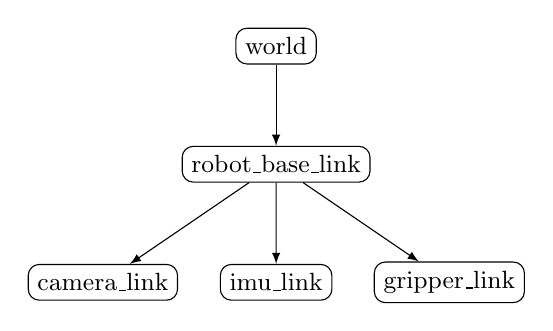
\begin{tikzpicture}[
        level 1/.style={sibling distance=3.5cm},
        level 2/.style={sibling distance=2.2cm}, % Adjusted spacing
        edge from parent/.style={draw, -latex},
        every node/.style={draw, rectangle, rounded corners, text centered, font=\small} % Made font slightly smaller for compactness
    ]
    \node {world}
        child { node {robot\_base\_link}
            child { node {camera\_link} }
            child { node {imu\_link} }
            child { node {gripper\_link} }
        };
    \end{tikzpicture}
    \caption{A simplified example of a ROS~2 transform tree (tf tree). The library manages the hierarchical relationships, allowing a program to easily calculate the transform from the \texttt{camera\_link} to the \texttt{world} frame, for example.}
    \label{fig:tf_tree_concept}
\end{figure}

In the architecture of this thesis, ROS~2 serves as the central \textbf{data backbone}, a concept adapted from digital engineering that describes an integrated communication layer for all relevant system knowledge \cite{perzylo2020backbone}. This "glue" connects the physical EMARO robot, its tracking system, and the virtual Unity environment. The digital twin of the EMAROS robot subscribes to ROS~2 topics to receive real-time data from the physical world, allowing it to synchronize its state through this communication layer \cite{singh2024unity}. For this project, the high-performance \texttt{ros2-for-unity} asset by Robotec.AI is used \cite{Rob24}. This solution is particularly advantageous because it does not bridge the communication but instead implements the ROS~2 middleware stack (RCL and below) directly within Unity. This means that entities within the simulation become "native" ROS~2 nodes, allowing them to respect Quality of Service (QoS) settings and achieve significantly lower latencies than bridged solutions \cite{Rob24}.

For advanced navigation tasks for both the physical robot and its virtual counterpart, this thesis utilizes \textbf{Navigation2 (Nav2)}, the official, next-generation autonomous navigation framework for ROS~2 \cite{macenski2020marathon2}. Nav2 was built from the ground up to orchestrate planning, control, and recovery tasks using configurable Behavior Trees, which are highly modular and can be modified at runtime to create unique navigation behaviors \cite{macenski2020marathon2}. At its core, Nav2 separates the task of navigation into two main components: a \textbf{global planner}, which finds an acceptable, long-range route through the environment, and a \textbf{local trajectory planner} (or controller), which generates velocity commands to follow that route while reacting to immediate obstacles \cite{macenski2023survey}. By leveraging the Nav2 stack, a high-level goal (e.g., a coordinate in the environment) can be sent via a ROS~2 action to either the physical EMARO robot or the purely virtual model, and the system will autonomously handle all complex path planning and collision avoidance.

\section{Simulation Engines for Robotics}
\label{sec:sim_engines}

Selecting the appropriate simulation engine is a foundational decision for the architecture of a Digital Twin. The simulator must serve as a synchronized virtual replica of the physical system, requiring a platform that balances computational efficiency with environmental realism \cite{Singh2025}. For this project, the selection process is driven by specific criteria derived from the requirements of Industry 5.0 applications: Visual Fidelity, Physics Accuracy, Native VR/AR Support, and the balance between Community Support and Learning Curve \cite{Gonzalez2025}.

\subsection{Traditional Robotics Simulators}
\textbf{Gazebo} is the most widely used simulator for Industry 4.0 applications due to its deep integration with ROS and its open-source nature \cite{Gonzalez2025}. It provides detailed physics simulations and sensor data emulation, making it ideal for precise engineering applications \cite{Singh2025}. However, while Gazebo benefits from a vast community and extensive documentation, it possesses notable limitations regarding visualization. Its rendering quality is described as "moderate," lacking the photorealism required for immersive Extended Reality (XR) experiences \cite{dosSantos2025}. Furthermore, studies note that Gazebo presents a steep learning curve for new users due to its complex configuration and less intuitive user interface compared to modern commercial tools \cite{Singh2025, Gonzalez2025}.

\textbf{Webots} is another prominent open-source platform, valued for its cross-platform support and extensive library of robot models \cite{Kargar2024}. While efficient for educational purposes, its rendering capabilities lag behind modern game engines, making it less suitable for high-fidelity XR visuals.

\subsection{Alternative Physics-Based Simulators}
Several other simulators were identified in the literature but were deemed less suitable for the specific XR requirements of this thesis. \textbf{CoppeliaSim (formerly V-REP)} is widely used for automation but offers limited physics realism compared to high-end tools and suffers from scalability constraints \cite{Gonzalez2025}. \textbf{MuJoCo} is highly regarded for contact-rich tasks and Reinforcement Learning (RL) but focuses almost exclusively on physics stability rather than visualization, lacking the built-in XR frameworks necessary for Mixed Reality interaction \cite{Gonzalez2025}.

\subsection{High-Fidelity and Game-Based Engines}
To address the visualization limitations of traditional simulators, the robotics community has increasingly adopted game engines.

\textbf{NVIDIA Isaac Sim} represents the state-of-the-art in industrial simulation, offering photorealism (ray-tracing) and advanced GPU-accelerated physics via PhysX \cite{dosSantos2025}. It excels in generating synthetic data for AI perception \cite{Kargar2024}. However, Isaac Sim imposes a high hardware barrier, strictly requiring high-end NVIDIA RTX GPUs \cite{dosSantos2025}. Additionally, as a proprietary platform, it limits accessibility for educational contexts compared to open-source or widely accessible game engines.

\textbf{Unreal Engine} is renowned for "best-in-class" photorealistic visuals and the ability to handle massive open-world environments \cite{Gonzalez2025}. However, it presents a steep learning curve due to its reliance on C++, making it less accessible for rapid prototyping compared to alternatives like Unity \cite{Coronado2023}.

\textbf{Unity Engine} has emerged as the dominant platform for Industry 5.0 applications, specifically those focusing on HRI and XR \cite{Gonzalez2025}. It offers a balance of high-fidelity graphics and a robust physics engine (PhysX) \cite{Singh2025}. Unity is recognized for its mature XR ecosystem and massive asset store, which significantly lowers the barrier to entry for developers. Literature highlights that Unity's user-friendly interface and supportive community facilitate a smoother learning curve compared to Gazebo or Unreal, particularly for users without deep C++ expertise \cite{Singh2025, Coronado2023}.

Crucially, Unity does not support ROS~2 natively out-of-the-box. Integration must be achieved through external plugins. This thesis utilizes the \textbf{ROS2 For Unity} plugin, available via GitHub from Robotec.AI \cite{Rob24}. This asset provides a high-performance communication solution by loading the ROS~2 middleware stack (RCL layer) directly into the Unity engine. Unlike bridged solutions, this allows simulation entities to function as "native" ROS~2 nodes within the Unity environment, respecting Quality of Service (QoS) settings and achieving significantly lower latencies \cite{Rob24}.

\subsection{Comparison and Selection}
Table \ref{tab:sim_comparison} summarizes the capabilities of these engines.

\begin{table}[h]
\centering
\caption{Comparison of Simulation Platforms for Mixed Reality Digital Twins \cite{Gonzalez2025, Kargar2024, Singh2025, Coronado2023}.}
\label{tab:sim_comparison}
\resizebox{\textwidth}{!}{%
\begin{tabular}{|l|c|c|c|c|}
\hline
\textbf{Feature} & \textbf{Gazebo} & \textbf{Isaac Sim} & \textbf{Unreal Engine} & \textbf{Unity} \\ \hline
\textbf{Primary Use Case} & Control \& Navigation & AI \& Photorealism & Photorealism & HRI \& XR (VR/AR) \\ \hline
\textbf{Visual Fidelity} & Moderate & Very High & Very High & High \\ \hline
\textbf{Physics Engine} & ODE/Bullet/DART & PhysX 5 (GPU) & Chaos/PhysX & PhysX \\ \hline
\textbf{Learning Curve} & Steep & Advanced & Steep (C++) & Moderate (C\#) \\ \hline
\textbf{Community Support} & High (ROS specific) & Moderate & High (Gaming) & Very High (XR/Gaming) \\ \hline
\textbf{ROS 2 Integration} & Native & Bridge & Bridge & Plugin (Native Stack) \\ \hline
\textbf{Hardware Req.} & Low & Very High (RTX) & High & Moderate \\ \hline
\end{tabular}%
}
\end{table}

\subsubsection{Rationale for Using the Unity Engine}
Based on this analysis, **Unity** is selected as the core simulation engine. It provides the necessary XR framework for Mixed Reality \cite{Coronado2023} and offers superior visualization compared to Gazebo \cite{Gonzalez2025}. Furthermore, it balances accessibility with power; its C\# scripting and vast community support offer a more manageable learning curve than Unreal Engine \cite{Coronado2023}, while the \texttt{ros2-for-unity} plugin ensures high-performance, low-latency communication \cite{Rob24}.

\section{The VERA Framework and EMARO}
\label{sec:emaro}

The capabilities of the VERA framework were demonstrated using a specific hardware testbed, the EMARO (Educational Modular Autonomous Robot Osnabrück) \cite{Geh24}. EMARO is a mobile, autonomous, and modular mini-robot developed at Osnabrück University, designed specifically for teaching and research in robotics, artificial intelligence, and computer engineering \cite{Geh24}.

The robot's hardware architecture is modular, based on three main Printed Circuit Boards (PCBs): a \textbf{Host-PCB} that integrates the compute module, a \textbf{Power-PCB} for energy management and motor control, and a \textbf{Base-PCB} for integrating ground and distance sensors \cite{Geh24}. The variant used in the original VERA thesis was equipped with a Raspberry Pi Compute Module 4, an Inertial Measurement Unit (IMU) for orientation, and two wide-angle cameras configured for stereo vision applications \cite{Geh24}. The EMARO robot is shown in Figure \ref{fig:emaro_robot}.

\begin{figure}[h]
    \centering
    % \includegraphics[width=0.4\textwidth]{figures/Geh24_Fig3-1.png}
    \caption[The EMARO robot.]{The EMARO (Educational Modular Autonomous Robot Osnabrück) platform used as the physical testbed for the VERA framework. Adapted from \cite{Geh24}.}
    \label{fig:emaro_robot}
\end{figure}

Critically for its integration, the entire system, including the EMARO, operates on the Robot Operating System 2 (ROS 2) \cite{Geh24}. Within the original VERA framework, EMARO navigated the projected environment autonomously by employing a camera-based, OpenCV line-following algorithm \cite{Geh24}. This \texttt{pathfinder} node processed the camera feeds to detect the projected line, calculate its centroid, and publish steering commands to the \texttt{/cmd\_vel} topic, enabling the robot to follow the path \cite{Geh24}. Data from the robot's IMU and system status (like CPU and RAM usage) were also published to ROS 2 topics, where VERA's visualizer could subscribe to them for AR projections \cite{Geh24}.

\subsection{Original VERA System Architecture}
\label{sec:vera_architecture}
The software architecture of the original VERA framework was built on ROS 2 and consisted of three main components: a positioning system (VEPS), an environment manager, and a dual-instance visualization system \cite{Geh24}. The interaction between these components, as described in the original thesis, is shown in Figure \ref{fig:vera_sw_architecture}.

\begin{figure}[h]
    \centering
    % \includegraphics[width=1.0\textwidth]{figures/Geh24_Fig4-4.png}
    \caption[Original VERA software components.]{The software architecture of the original VERA framework, showing the data flow between the EMARO, the 3D Camera, the core VERA nodes (VEPS, Manager, Visualizer), and RViz. Adapted from \cite{Geh24}.}
    \label{fig:vera_sw_architecture}
\end{figure}

\subsubsection{Virtual Environment Positioning System (VEPS)}
The first component, the Virtual Environment Positioning System (VEPS), was responsible for the real-time localization of the EMARO \cite{Geh24}. This system did not use traditional vision, but instead relied on depth data \cite{Geh24}. It utilized an Allied Vision Ruby 3D stereo camera, mounted above the test area, to capture a 3D point cloud of the environment \cite{Geh24}.

This point cloud data was processed in several steps. First, it was filtered to remove the ground plane and sensor noise, isolating the points corresponding to the robot \cite{Geh24}. Second, the \textbf{Median Absolute Deviation (MAD)} algorithm was applied to the remaining points to statistically find their center \cite{Geh24}. This calculated centroid was used as the robot's 2D $(x, y)$ position. This position was then smoothed using a Kalman filter and published as a ROS 2 transform (\texttt{/tf}) for other nodes to consume \cite{Geh24}. The evaluation of VEPS showed it could achieve processing times under 5ms at a 30 FPS update rate \cite{Geh24}.

\subsubsection{Virtual Environment Manager}
The second component was the Environment Manager, which acted as the central "brain" of the simulation \cite{Geh24}. This C++ ROS 2 node was responsible for parsing, managing, and updating the state of the virtual world \cite{Geh24}. It would load environments from standard Gazebo-compatible \textbf{\texttt{world.sdf}} files, which defined the models, poses, and custom properties (e.g., "movable" or "removable") of all virtual objects \cite{Geh24}.

The manager ran a main loop on a 50ms timer \cite{Geh24}. In each loop, it would look up the robot's current position (published by VEPS) and perform collision checks between the robot and all spawnable objects in the environment \cite{Geh24}. If a collision was detected, the manager would update the object's state (e.g., marking it for removal) and publish these changes to the visualizers using ROS 2 \textbf{\texttt{MarkerArray}} messages over the \texttt{/objects} topic \cite{Geh24}. This node was also responsible for path tracking, recording the robot's position history and publishing it as a \texttt{/path} message for the AR visualization \cite{Geh24}.

\subsubsection{Visualization System (RViz and Pygame)}
Finally, the visualization system consisted of two separate, synchronized instances that both subscribed to the manager's \texttt{/objects} and \texttt{/path} topics \cite{Geh24}.

\begin{enumerate}
    \item \textbf{RViz:} The standard ROS visualization tool, RViz, was used as a 3D simulation interface \cite{Geh24}. It provided a detailed 3D view for debugging and monitoring, displaying the robot's digital twin (from its URDF model), the virtual objects, the robot's driven path, and other debug data like the VEPS point cloud \cite{Geh24}. An example of the RViz interface from the original thesis is shown in Figure \ref{fig:vera_rviz_view}.
    
    \begin{figure}[h]
        \centering
        % \includegraphics[width=0.7\textwidth]{figures/Geh24_Fig4-10.png}
    \caption[RViz 3D view in VERA.]{The RViz simulation interface in the original VERA framework, showing a 3D view of the virtual objects (green), the EMARO's digital model (grey), and its driven path. Adapted from \cite{Geh24}.}
        \label{fig:vera_rviz_view}
    \end{figure}
    
    \item \textbf{2D Projector Node:} This was the custom-built component responsible for projecting the virtual world onto the physical floor \cite{Geh24}. This ROS 2 node, written in Python, used the \textbf{Pygame library} to render a 2D orthogonal, top-down view of the environment \cite{Geh24}. It subscribed to the manager's topics to draw all the virtual objects and the robot's path \cite{Geh24}. This node also rendered the AR-like features, such as a status display (showing EMARO's CPU and RAM usage) that was projected onto the floor behind the robot, following its position and orientation in real-time \cite{Geh24}. The final rendered output of this Pygame node is shown in Figure \ref{fig:vera_pygame_view}.

    \begin{figure}[h]
        \centering
        % \includegraphics[width=0.7\textwidth]{figures/Geh24_Fig4-11.png}
    \caption[Pygame 2D rendered projection in VERA.]{The 2D orthogonal view rendered by the custom Pygame visualizer, as it would be sent to the projector. It displays the objects (green), the robot's position (red dot), its path (cyan), and the AR status display. Adapted from \cite{Geh24}.}
        \label{fig:vera_pygame_view}
    \end{figure}
\end{enumerate}
\subsection{Platform Changes and Identified Limitations}
\label{sec:vera_limitations}

While the \texttt{[Geh24]} thesis established the VERA framework's concept, this thesis builds upon an evolved version of the platform and directly addresses the specific software limitations documented in the original work.

\subsubsection{Changes of the Positioning System}
The VERA platform is modular, and its components have been iterated upon. The point-cloud-based VEPS \cite{Geh24} is no longer in use. Instead, the platform for this thesis employs a more robust, marker-based tracking system. This system, developed in a separate bachelor's thesis \cite{Your_BA_Thesis_Citation}, uses ArUco markers and multiple cameras to provide a high-precision 6D pose (position and orientation) of the robot, which it publishes over a ROS 2 topic. This thesis consumes this pose data as a service. The internal implementation of the ArUco tracking system itself is outside the scope of this project.

\subsubsection{Identified Limitations of the Original Software}
While the positioning system was updated, the core software limitations of the original VERA manager and visualizer remained. These limitations, explicitly documented in the \texttt{[Geh24]} thesis, form the primary justification for this work:

\begin{itemize}
    \item \textbf{Lack of Realistic Physics:} The custom-built environment manager was a significant limitation as it did not include an enhanced physics engine for realistic interactions. The \texttt{[Geh24]} thesis concludes by listing the "integration of enhanced physics into the manager's implementation" as a primary direction for future work \cite{Geh24}.
    
    \item \textbf{Performance and Scalability Bottlenecks:} The evaluation of the \textbf{Pygame-based 2D visualizer} revealed significant performance limitations \cite{Geh24}. In scenarios with a high number of object updates (e.g., >800--1250 objects), the system's responsiveness failed, and marker latencies were observed to "spike into seconds" \cite{Geh24}. The original thesis identified the cause of this bottleneck: the visualizer's message queue could not process the high frequency of individual marker messages, leading to "delayed and incomplete updates" \cite{Geh24}.
    
    \item \textbf{Limited Interaction Modalities:} Finally, while the AR projections were successful, more immersive and interactive modalities were not implemented. The \texttt{[Geh24]} thesis concludes by suggesting a "virtual reality integration to interact with the simulated environment via VR headsets" as another "possible extension" of the system \cite{Geh24}.
\end{itemize}

These three documented limitations---a lack of physics, a non-scalable custom visualizer, and the absence of VR interaction---are the specific problems this thesis solves by replacing VERA's custom manager and Pygame visualizer with the Unity Engine.